This calculator employs an event-based Monte Carlo simulation approach to
probabilistic risk assessment in order to estimate the loss distribution for
individual \glspl{asset} and aggregated loss distribution for a spatially
distributed portfolio of \glspl{asset} within a specified time period. The
calculator requires the definition of an \gls{exposuremodel}, a
\gls{vulnerabilitymodel} for each loss type of interest with
\glspl{vulnerabilityfunction} for each taxonomy represented in the
\gls{exposuremodel}, and a \glsdesc{acr:ses} (also known as a
\textit{synthetic catalog}) representative of the seismicity of the region
over the specified time period. Loss curves and loss maps can currently be
calculated for five different loss types using this calculator: structural
losses, nonstructural losses, contents losses, downtime losses, and occupant
fatalities.

As an alternative to computing the \glspl{acr:gmf} with \glsdesc{acr:oqe},
users can also provide their own sets of \glspl{acr:gmf} as input to the
event-based risk calculator, starting from \gls{acr:oqe28}.

The main results of this calculator are loss
exceedance curves for each \gls{asset}, which describe the probability of
exceedance of different loss levels over the specified time period, and loss
maps for the region, which describe the loss values that have a given
probability of exceedance over the specified time period. Aggregate loss
exceedance curves can also be produced using this calculator; these
describe the probability of exceedance of different loss levels for all
\glspl{asset} in the portfolio. Finally, event loss tables can be produced
using this calculator; these tables describe the total loss across the
portfolio for each seismic event in the \gls{acr:ses}.

This calculator relies on the probabilistic event-based hazard calculator,
which simulates the seismicity of the chosen time period $T$ by producing a
\gls{acr:ses}. For each \gls{rupture} generated by a \gls{seismicsource}, the
number of occurrences in the given time span $T$ is simulated by sampling the
corresponding probability distribution as given by $P_{rup}(k | T)$. A
\gls{acr:ses} is therefore a \textit{sample} of the full population of
\glspl{rupture} as defined by a \glsdesc{acr:ssm}. Each \gls{rupture} is
present zero, one or more times, depending on its probability. Symbolically,
we can define a \gls{acr:ses} as:
\begin{align}
SES(T) = \left\{k \times rup,\;k\sim P_{rup}(k | T)\;\;\forall\;rup\;in\;Src\;\forall\;Src\;in\;SSM\right\}
\end{align}
where $k$, the number of occurrences, is a random sample of $P_{rup}(k | T)$,
and $k \times rup$ means that \gls{rupture} $rup$ is repeated $k$ times in the
\gls{acr:ses}.

For each \gls{rupture} or event in the \glspl{acr:ses}, a spatially correlated
\gls{acr:gmf} realisation is generated, taking into consideration both the
inter-event variability of ground motions, and the intra-event residuals
obtained from a spatial correlation model for ground motion residuals (if one 
is specified in the job file). The use of logic trees allows for the 
consideration of uncertainty in the choice of a \glsdesc{acr:ssm}, and in the 
choice of \glspl{groundmotionmodel} for the different tectonic regions.

For each \gls{acr:gmf} realization, a loss ratio is sampled for every
\gls{asset} in the \gls{exposuremodel} using the provided probabilistic
\gls{vulnerabilitymodel}, taking into consideration the correlation model for
vulnerability of different \glspl{asset} of a given taxonomy. Finally loss
exceedance curves are computed for ground-up losses.

The required input files required for running a probabilistic stochastic
event-based risk calculation and the resulting output files are depicted in
Figure~\ref{fig:io-structure-event-based-risk}

\begin{figure}[ht]
\centering
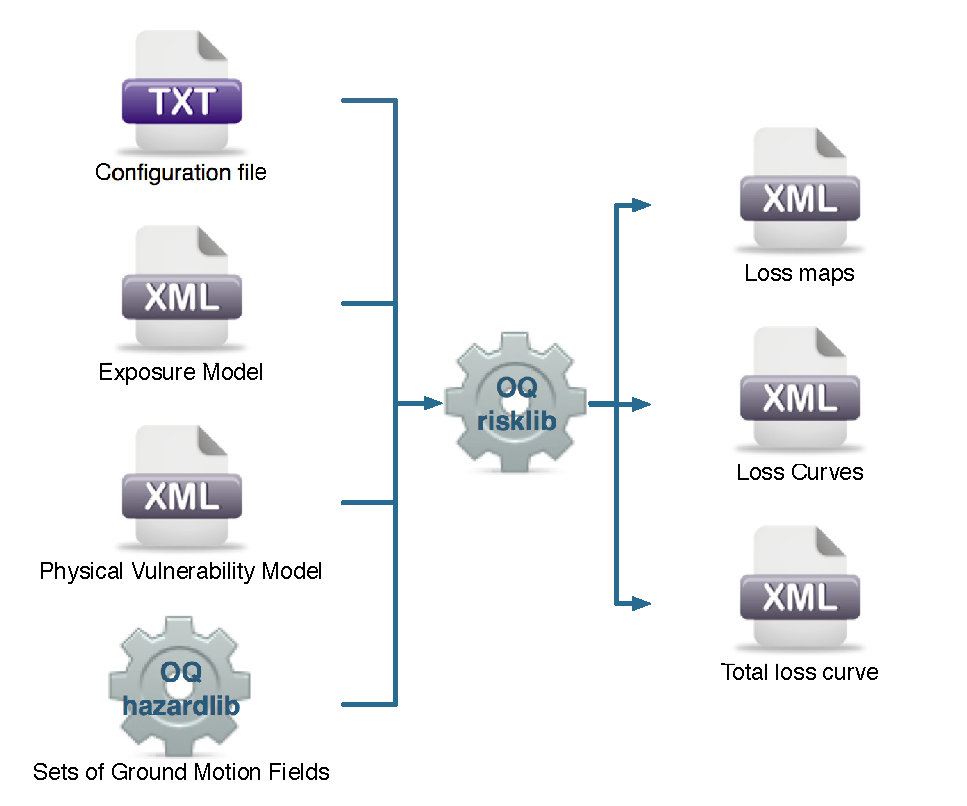
\includegraphics[width=9cm,height=7cm]{figures/risk/io-structure-event-based-risk.pdf}
\caption{Probabilistic Event-based Risk Calculator input/output structure.}
\label{fig:io-structure-event-based-risk}
\end{figure}
